\section{Captive Portal}

\subsection{Algemeines}
Als Captive Portal (zu deutsch etwa „Umleitung auf ein Web-Portal“) wird eine Website bezeichnet,
die dafür verwendet wird Authentifizierungen durchzuführen, meistens findet sie in WLANs
Einsatz. In unserem Fall dient sie dem Login auf einer HTTP-Seite um sich beim RADIUS-Server
einzuloggen. \cite{chilli0}

\subsection{Funktionsweise}
Prinzipiell ist die Funktionsweise relativ simpel. Man benötigt lediglich einen Webserver und eine
Firewall, in unserem Fall Apache2 und iptables. Wenn nun ein Benutzer in ein WLAN-Netzwerk
möchte, wird erst einmal der komplette Netzwerkverkehr ignoriert, bis er einen Browser öffnet.
Dieser Zugriff wird immer auf das Captive Portal weitergeleitet, sodass der Benutzer immer zu der
Login-Seite kommt. Je nach Anwendungsfall können dort dann auch Bezahlsysteme implementiert
werden oder Nutzungsbedingungen die akzeptiert werden müssen.\\
Es gibt verschiedene Möglichkeiten wie die Umleitung von Statten gehen kann, durchgesetzt hat
sich aufgrund verschiedener sicherheitstechnischer Aspekte die Umleitung via HTTP (direkte IP-
sowie DNS-Umleitungen sind aufgrund des dann nicht mehr gültigen DNSSEC-Zertifikats nicht
möglich). \cite{chilli1}
\newpage
\subsection{CoovaChilli}
Allgemeines:\\
CoovaChilli ist ein open-source Tool das unter der GNU General Public License 3 veröffentlich wurde und frei zugänglich ist. Es bietet eine Zugriffskontrolle als Captive Portal und liefert die dafür benötigten HTML/CSS/Javascript Dateien. Es basiert auf dem mittlerweile nicht mehr unterstützten Projekt CoovaSpot und funktioniert mit dem RADIUS-Protokoll.\\
~\\
Funktionsweise:
\begin{figure}[ht]                                                                              
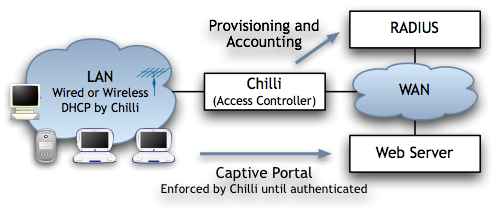
\includegraphics[width=\textwidth]{pictures/Tom/Chilli}
\caption{CoovaChilli Funktionsweise}
Quelle: \cite{chilli2}
\end{figure}
~\\
Wie in der Abbildung oberhalb zu erkennen bildet CoovaChilli die Instanz zwischen dem Access-
Point des Netzwerks und der Netzwerkinfrastruktur dahinter (in unserem Fall laufen Netzwerk-
Access-Server, also dem WLAN-AP, CoovaChilli und der RADIUS-Server auf der gleichen Maschine).
Will ein Benutzer nun ins Internet verbindet er sich wahlweise per LAN oder WLAN mit dem AP,
ruft den Browser auf und wird auf das Captive Portal auf dem Webserver weitergeleitet. Beim
Login kommuniziert CoovaChilli mit dem RADIUS-Server, bei erfolgreichem Login wird der
Internetzugang für den Benutzer freigegeben.
\newpage
Installation:\\

